\subsection{When does stochastic planning matter? (Experiment I2)}
To find the conditions under which uncertainty changes the decision, we repeated the comparison with export
capacity limited to 300~MW. Surplus PV must then be stored, absorbed by the reservoir or curtailed. We also
raised the budget, so that PV saturates before the budget binds (Table~\ref{tab:i2}). With 900~MW of export
capacity the stochastic and deterministic plans remain identical at every risk weight (VSS = 0). With
restricted exports and risk-neutral planning ($\lambda=0$), the stochastic plan adds slightly more PV than the
deterministic one (+26~MW at 1{,}000~MEUR, +75~MW at 1{,}500~MEUR), and the VSS is only 0.2--0.3~MEUR/yr. With
restricted exports, a 1{,}500~MEUR budget and $\lambda=1$, the decision changes qualitatively. The risk-averse
plan adds 1{,}520~MW of PV, 230~MW of \emph{wind} and a 30~MW / 66~MWh battery. The deterministic plan adds
1{,}232~MW of PV only. In the representative-week model the risk-averse plan raises expected cost by
7.8~MEUR/yr and lowers CVaR$_{0.9}$ of operating cost by 79~MEUR/yr (from 292 to 213); the risk-adjusted VSS is
71.5~MEUR/yr. Full-year chronological re-evaluation of the two plans confirms the trade-off. Expected total
cost is higher by 15.1~MEUR/yr (74.6 vs 59.5), CVaR$_{0.9}$ of operating cost is lower by 74.5~MEUR/yr (208.2
vs 282.7), and neither plan has any unserved energy. The hedge is mainly wind rather than storage. Once PV saturates
under the export limit, wind is the cheapest remaining way to cut imports in the high-price stress scenarios.
We did not decompose this mechanism further, for example by wind--PV correlation or season. Stochastic, risk-aware planning therefore matters when a no-regret resource
saturates because its surplus cannot leave the system. In that regime the choice among the remaining resources
depends on the tail scenarios.

\IfFileExists{tables/tab_i2.tex}{\begin{table}[htbp]
\centering
\scriptsize
\caption{Experiment I2: stochastic (RP) versus deterministic-plan evaluation (EEV) under restricted and full export capacity. Additions as PV/wind MW / battery MW/MWh; E = expected total annualised cost, CVaR$_{0.9}$ of operating cost and risk-adjusted VSS in MEUR/yr (representative weeks, water-value boundaries).}
\label{tab:i2}
\begin{adjustbox}{max width=\linewidth}
\begin{tabular}{lrrrrrrrrr}
\toprule
Export MW & Budget & $\lambda$ & Stoch. adds & Det. adds & E RP & E EEV & CVaR RP & CVaR EEV & VSS \\
\midrule
300 & 1\,000 & 0 & 1\,258/0/0/0 & 1\,232/0/0/0 & 62.0 & 62.1 & 288.1 & 292.0 & 0.2 \\
300 & 1\,000 & 1 & 1\,258/0/0/0 & 1\,232/0/0/0 & 62.0 & 62.1 & 288.1 & 292.0 & 4.1 \\
300 & 1\,500 & 0 & 1\,307/0/0/0 & 1\,232/0/0/0 & 61.8 & 62.1 & 281.1 & 292.0 & 0.3 \\
300 & 1\,500 & 1 & 1\,520/230/30/66 & 1\,232/0/0/0 & 70.0 & 62.1 & 212.7 & 292.0 & 71.5 \\
900 & 1\,500 & 0 & 1\,888/0/0/0 & 1\,888/0/0/0 & 12.9 & 12.9 & 170.2 & 170.2 & 0.0 \\
900 & 1\,500 & 1 & 1\,888/0/0/0 & 1\,888/0/0/0 & 12.9 & 12.9 & 170.2 & 170.2 & 0.0 \\
\bottomrule
\end{tabular}
\end{adjustbox}
\end{table}
}{}

\begin{figure}[htbp]
\centering
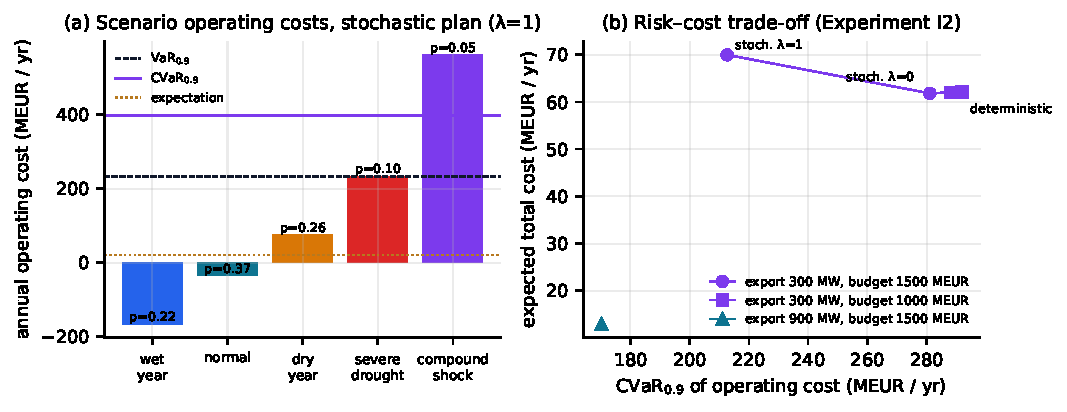
\includegraphics[width=\textwidth]{fig09_cvar.pdf}
\caption{(a) Annualised operating cost of the reference stochastic plan in each scenario, with probabilities, VaR$_{0.9}$,
CVaR$_{0.9}$ and the expectation. In the base case this plan is identical to the deterministic plan. (b) Expected total cost
versus CVaR$_{0.9}$ of operating cost for the deterministic plan and the stochastic plans ($\lambda=0,1$) in
Experiment~I2. Only with restricted exports and a large budget does risk aversion buy a material reduction in tail
cost.}
\label{fig:cvar}
\end{figure}
